\documentclass[12pt]{article}
\usepackage[english]{babel}
\usepackage[utf8]{inputenc}

\usepackage{geometry}
\geometry{
	letterpaper, 
	portrait, 
	top=.75in,
	left=.8in,
	right=.75in,
	bottom=.5in		} 	% Page Margins
	
%% additional packages for nice things
\usepackage{amsmath} 	% for most math
\usepackage{commath} 	% for abs
\usepackage{lastpage}	% for page count
\usepackage{amssymb} 	% for therefore
\usepackage{graphicx} 	% for image handling
\usepackage{wrapfig} 	% wrap figures
\usepackage[none]{hyphenat} % for no hyphenations
\usepackage{booktabs} 	% enhanced table qualities
\usepackage{array} 		% for >{} column characterisctis
\usepackage{physics} 	% for easier derivative \dv....
\usepackage{tikz} 		% for graphic@!
\usepackage{circuitikz} % for circuits!
\usetikzlibrary{arrows.meta} % for loads
\usepackage[thicklines]{cancel}	% for cancels
\usepackage{xcolor}		% for color cancels
\usepackage[per-mode=fraction]{siunitx} % for si units and num
\usepackage{fancyhdr} 	% for header
\usepackage{comment}	% for ability to comment out large sections
\usepackage{multicol}	% for multiple columns using multicols
\usepackage[framed,numbered]{matlab-prettifier} % matlab sytle listing
\usepackage{marvosym} 	% for boltsymbol lightning
\usepackage{pdflscape} 	% for various landscape pages in portrait docs.
\usepackage{float}
\usepackage{fancyvrb}	% for Verbatim (a tab respecting verbatim)
\usepackage{enumitem}	% for [resume] functionality of enumerate

%% package config 
\sisetup{output-exponent-marker=\ensuremath{\mathrm{E}}} % for engineer E
\renewcommand{\CancelColor}{\color{red}}	% for color cancels
\lstset{aboveskip=2pt,belowskip=2pt} % for more compact table
\def\arraystretch{1.4} % adjust size of arrays
%\arraycolsep=1.4pt\def
\setlength{\parindent}{0cm} % Remove indentation from paragraphs
\setlength{\columnsep}{0.5cm}
\lstset{
	style      = Matlab-editor,
	basicstyle = \ttfamily\footnotesize, % if you want to use Courier - not really used?
}
\renewcommand*{\pd}[3][]{\ensuremath{\dfrac{\partial^{#1} #2}{\partial #3}}} % for larger pd fracs
\renewcommand{\real}[1]{\mathbb{R}\left\{ #1 \right\}}	% for REAL symbol
\newcommand{\imag}[1]{\mathbb{I}\left\{ #1 \right\}}	% for IMAG symbol
\definecolor{m}{rgb}{1,0,1}	% for MATLAB matching magenta
	
%% custom macros
\newcommand\numberthis{\addtocounter{equation}{1}\tag{\theequation}} % for simple \numberthis command
\newcommand{\equal}{=} % so circuitikz can have an = in the labels
\newcolumntype{L}[1]{>{\raggedright\let\newline\\\arraybackslash\hspace{0pt}}m{#1}}
\newcolumntype{C}[1]{>{\centering\let\newline\\\arraybackslash\hspace{0pt}}m{#1}}
\newcolumntype{R}[1]{>{\raggedleft\let\newline\\\arraybackslash\hspace{0pt}}m{#1}}

%% Header
\pagestyle{fancy} % for header stuffs
\fancyhf{}
\rhead{Thad Haines \\ Page \thepage\ of \pageref{LastPage}}
\chead{Talking Points \\ Weeks of February 25 - March 4, 2019}
\lhead{Research \\ }
% spacing
\headheight 29 pt
\headsep 6 pt

\begin{document}
	\paragraph{Recent Progress:}
	\begin{enumerate}
		\item Given up on GE for API fixes or updates.
		
		\item SQL database for cross instance/code language communication concept proven.
		\subitem Involves using an SQL database as a common data resource. A timing schedule is  required so that a process doesn't 'step' on another process and cause concurrency issues.
		\subitem Using SQLite3 is may not be a great choice - it is not designed for 'fast' use but is included with python3 and ironpython.
		\subitem Other SQL database packages \textit{could} be explored - Must be compatible with Ipy32.
		
		\item AMQP (Advanced Message Queuing Protocol) for cross/instance code language communication concept proven. (suggested by Phil)
		\subitem Involves sending messages to an external service running on the local machine. These messages are then collected via code interfaces.
		\subitem Results are consistently faster than SQL method ($\approx$10-20 times faster)
		\subitem Unsure if it's best to use this alone, or in combination with a SQL database.
		
		\item AMQP SQL method for cross/instance code language communication concept proven.
		\subitem Provides consistently faster SQL access ($\approx$8-11 times faster than SQL only)
		\subitem Possibly the way to go - More forward development thinking required before decision.
		
		\item Read papers from the 70's by Mills, Taylor, and Cresap (surprisingly good).
		
		\item PSLF terminal output can be suppressed by EPCL command : \verb|dispar[0].noprint = 1|
		
		\item GitHub repository updated:
		\subitem \verb|https://github.com/thadhaines/| (SQL and AMQP tests also on GIT)
		
	\end{enumerate}
\paragraph{Current Tasks:}
	\begin{enumerate}
		\item Figure out how Python 3 is going to send data to, and receive data from, PSLF.
		\item Define Agent actions for AGC/LFC (ACE calculations), Shunt Control, $\beta$ calculation
		\item ODE solver == numpy / scipy \verb|odeint| in Python 3
		
		\item Continue experimenting with a multi-area model:\\
		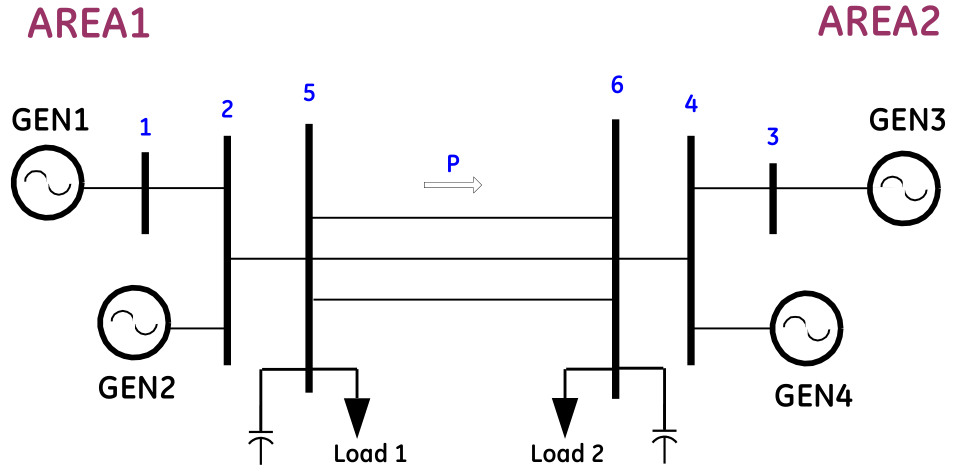
\includegraphics[width=.5\linewidth]{g4aSys}
		\item Investigate line current data (add branch section agents to model)
		%\subitem A FlowtabrDAO exists that can find flow between busses. A way to initialize bus connections between areas has yet to be devised.
		
		\item Refine data output - keep quickplotter in mind - Dictionary structure, variable naming, functionality, meta...
	\end{enumerate}
\pagebreak
\paragraph{Future Tasks:}(Little to No Progress since last time / Things coming down the pipe)
	\begin{enumerate}
		\item Add Ramp perturbance Agent
		
		\item An agent for every object: Shunt, SVD, Branch, Transformer, Power Plant, ...
		
		\item Think about having all simulation parameters be defined in one file that is fed into simulation. i.e. Have all perturbance, AGC, LTD, etc., related code in a text file so python doesn't have to be a 'user' thing.
		
		\item Package code into library and refactor (think of a nice name):\\
		Power System Long-Term Dynamic Simulation $\rightarrow$ PSLTDSim
		
		\item Investigate Runge-Kutta integration.. (probably inside scipy...)\\
		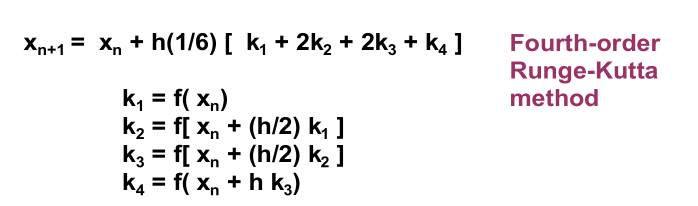
\includegraphics[width=.7\linewidth]{rk4}
		
		\item Enable multiple dyd files to overwrite / replace previously defined agents/parameters
		
		\item Identify System Slack bus programmatically (maybe just assume in first area?)
		\subitem or calculate system slack error differently... An average of slack error?
		
		%\subitem Can locate when only 1 Slack exists. If more than one Slack, maybe identify by generator with most busses under control? Proving more difficult than expected. Can identify in PSLF via the \verb|summ()| or \verb|isld()| commands. 
		
	\end{enumerate}
	\paragraph{Current Questions:}
	\begin{enumerate}
		
	%	\item Should another powerflow be computed once dynamic responses have been recorded to PSLF / python mirror? (as noted in CM 5h)
		
		\item Overview of planned PSLF scenarios? $\rightarrow$ Similar to Heredia but on MiniWecc Scale?
		
		\item Is there more available/relevant event data that may help us to verify simulations of specific instances (wind ramps or other behavior) that the novel research will focus on?\\ (Heredia paper data helpful for some wind ramp data context)
	\end{enumerate}
	\begin{comment}
 	place for comments
 	\paragraph{20 MW Load step Results:} Using ee554.sav case and only generator dynamics.\\
 	
 	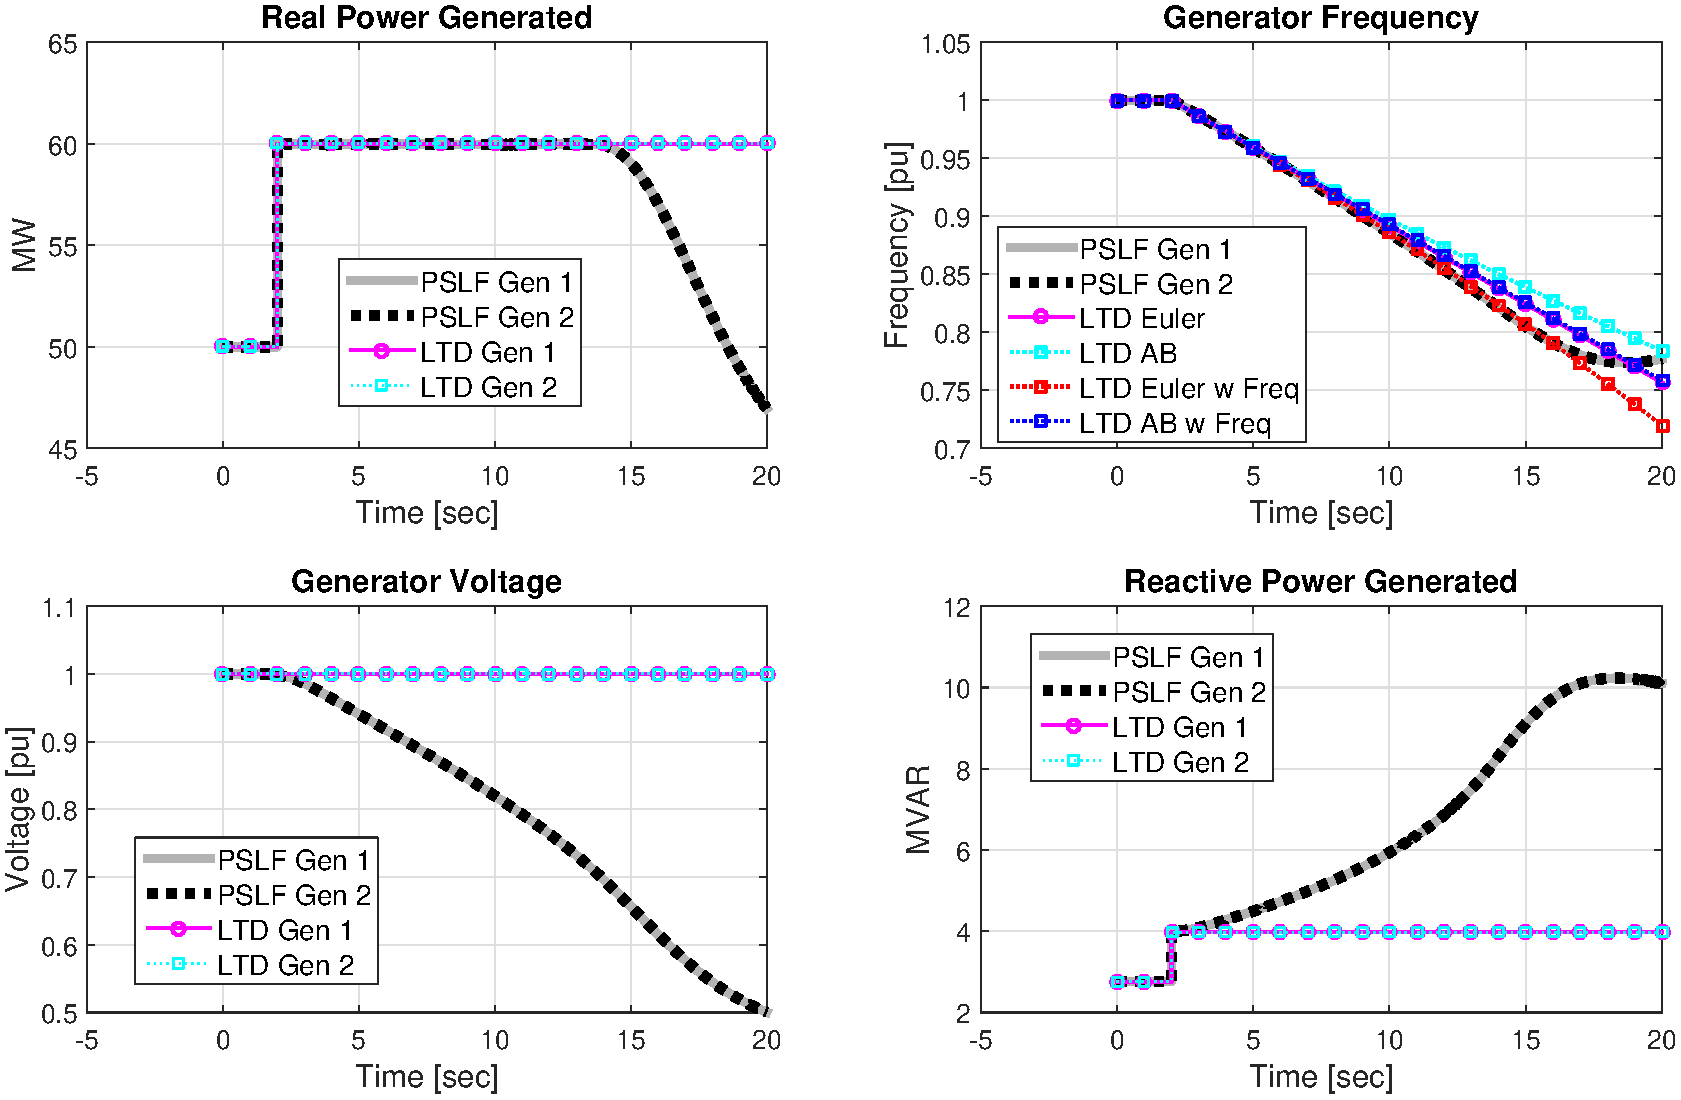
\includegraphics[width=\linewidth]{noGov_LTD01.pdf}
 	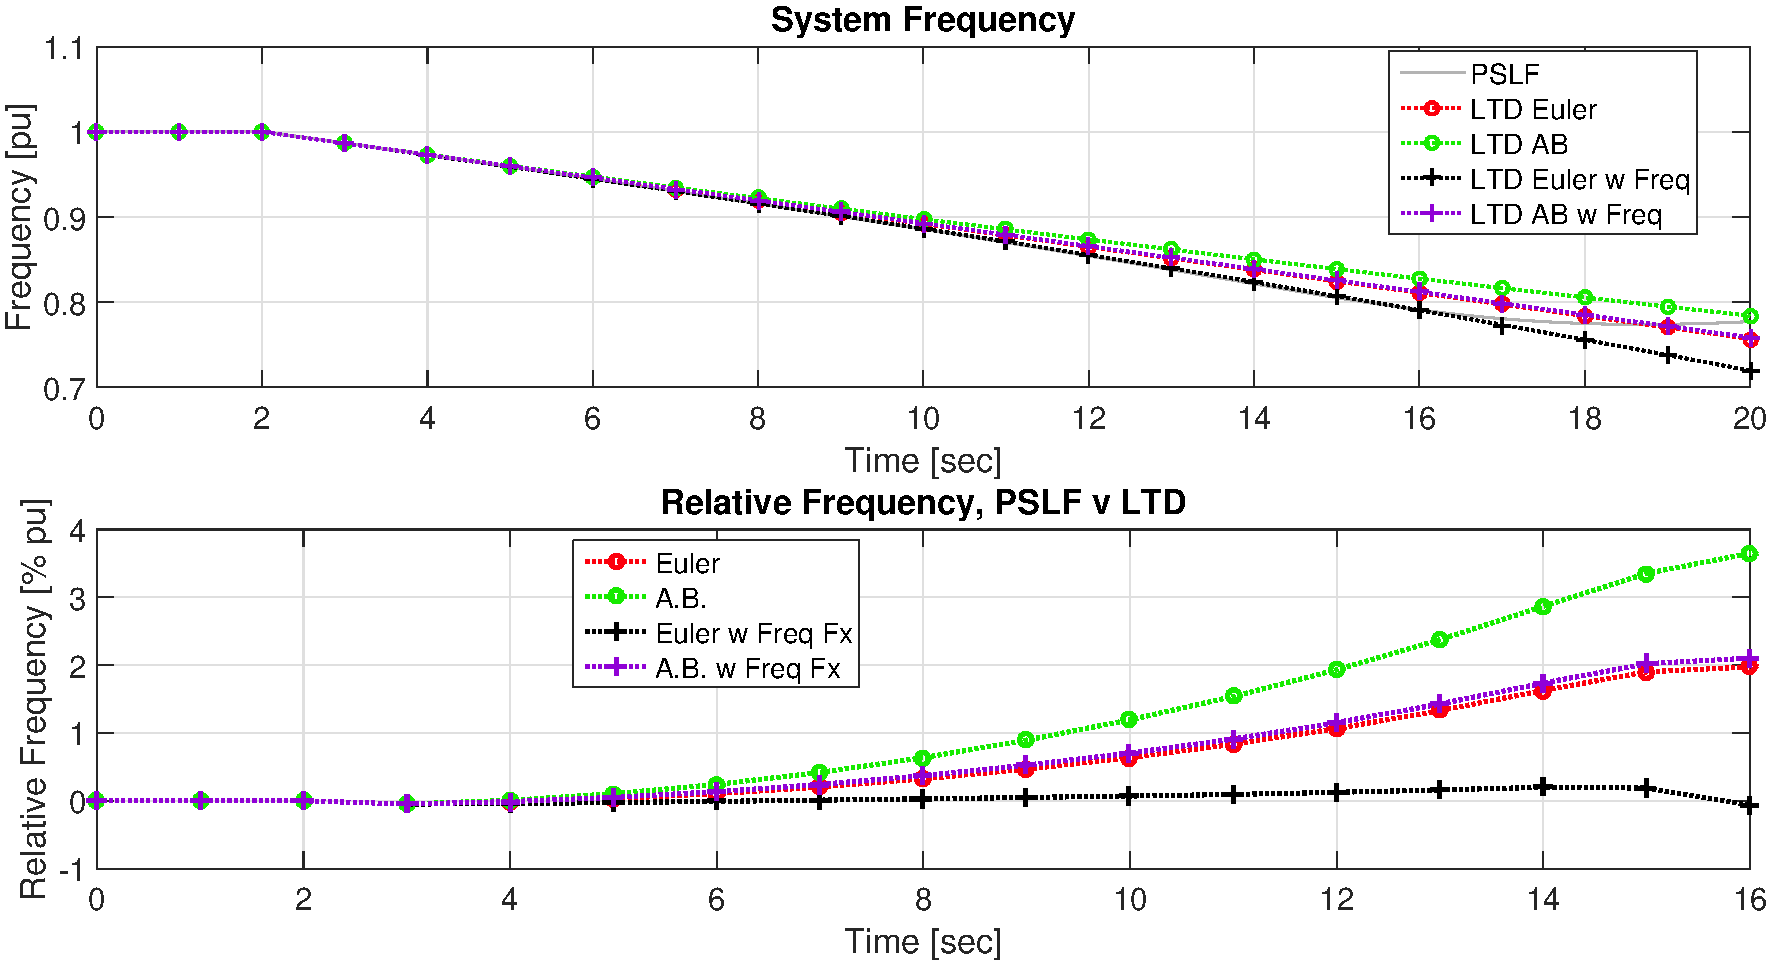
\includegraphics[width=\linewidth]{noGov_LTD04.pdf}

\pagebreak
\paragraph{EE544 Base System Results:}Stepping a 20 MW Load on at t=2 \vspace{1em}\\
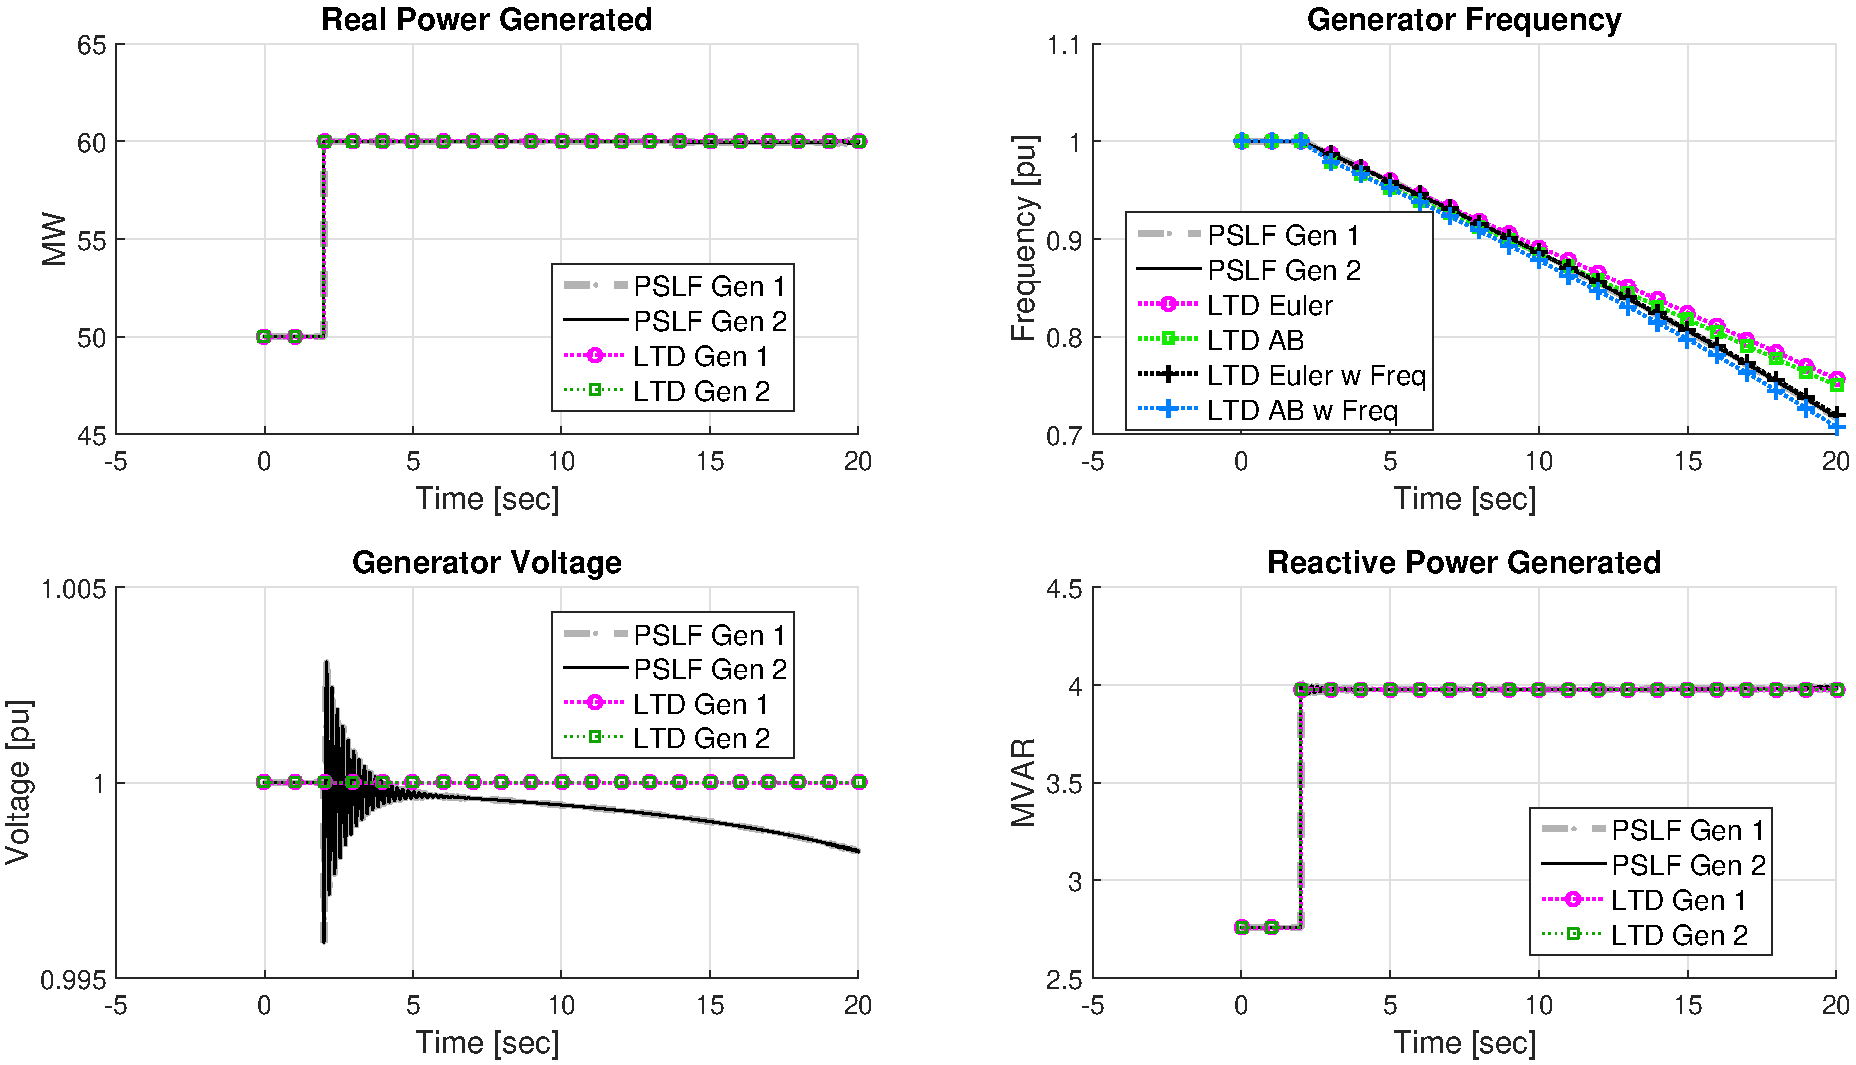
\includegraphics[width=\linewidth]{noGovExcLoadStepUpsys.pdf}
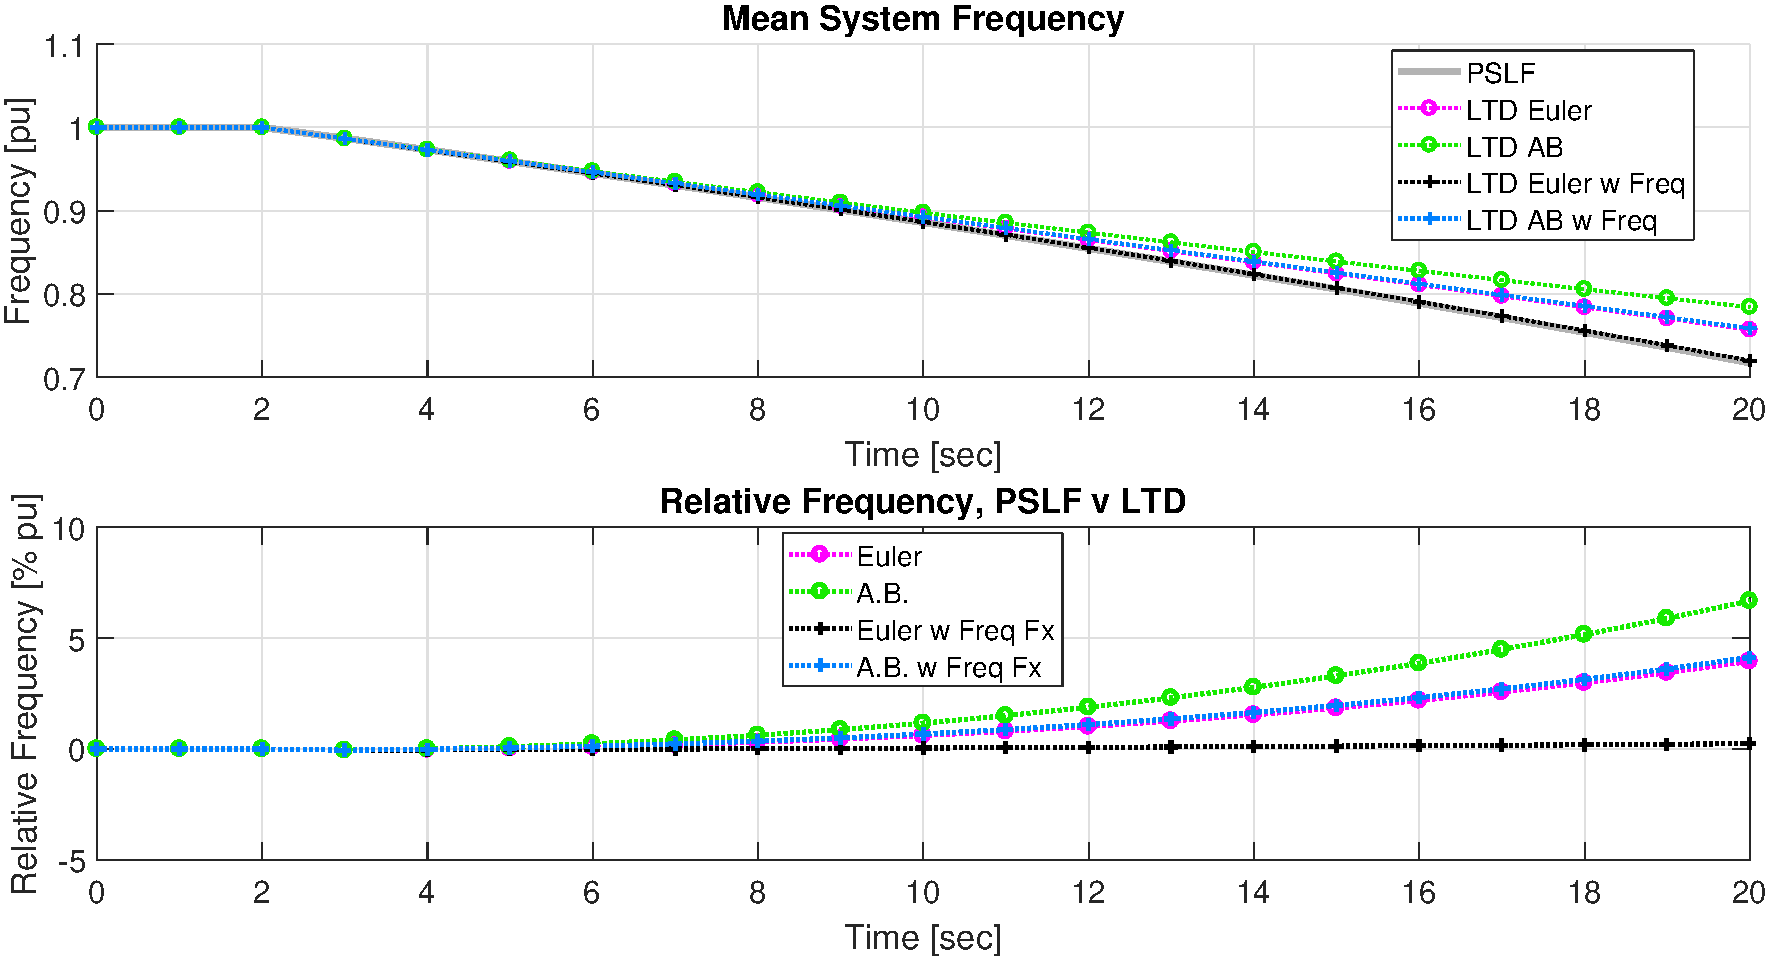
\includegraphics[width=\linewidth]{noGovExcLoadStepUpfreq}
\pagebreak \\
Stepping off a 20 MW Load at t=2 \vspace{1em}\\
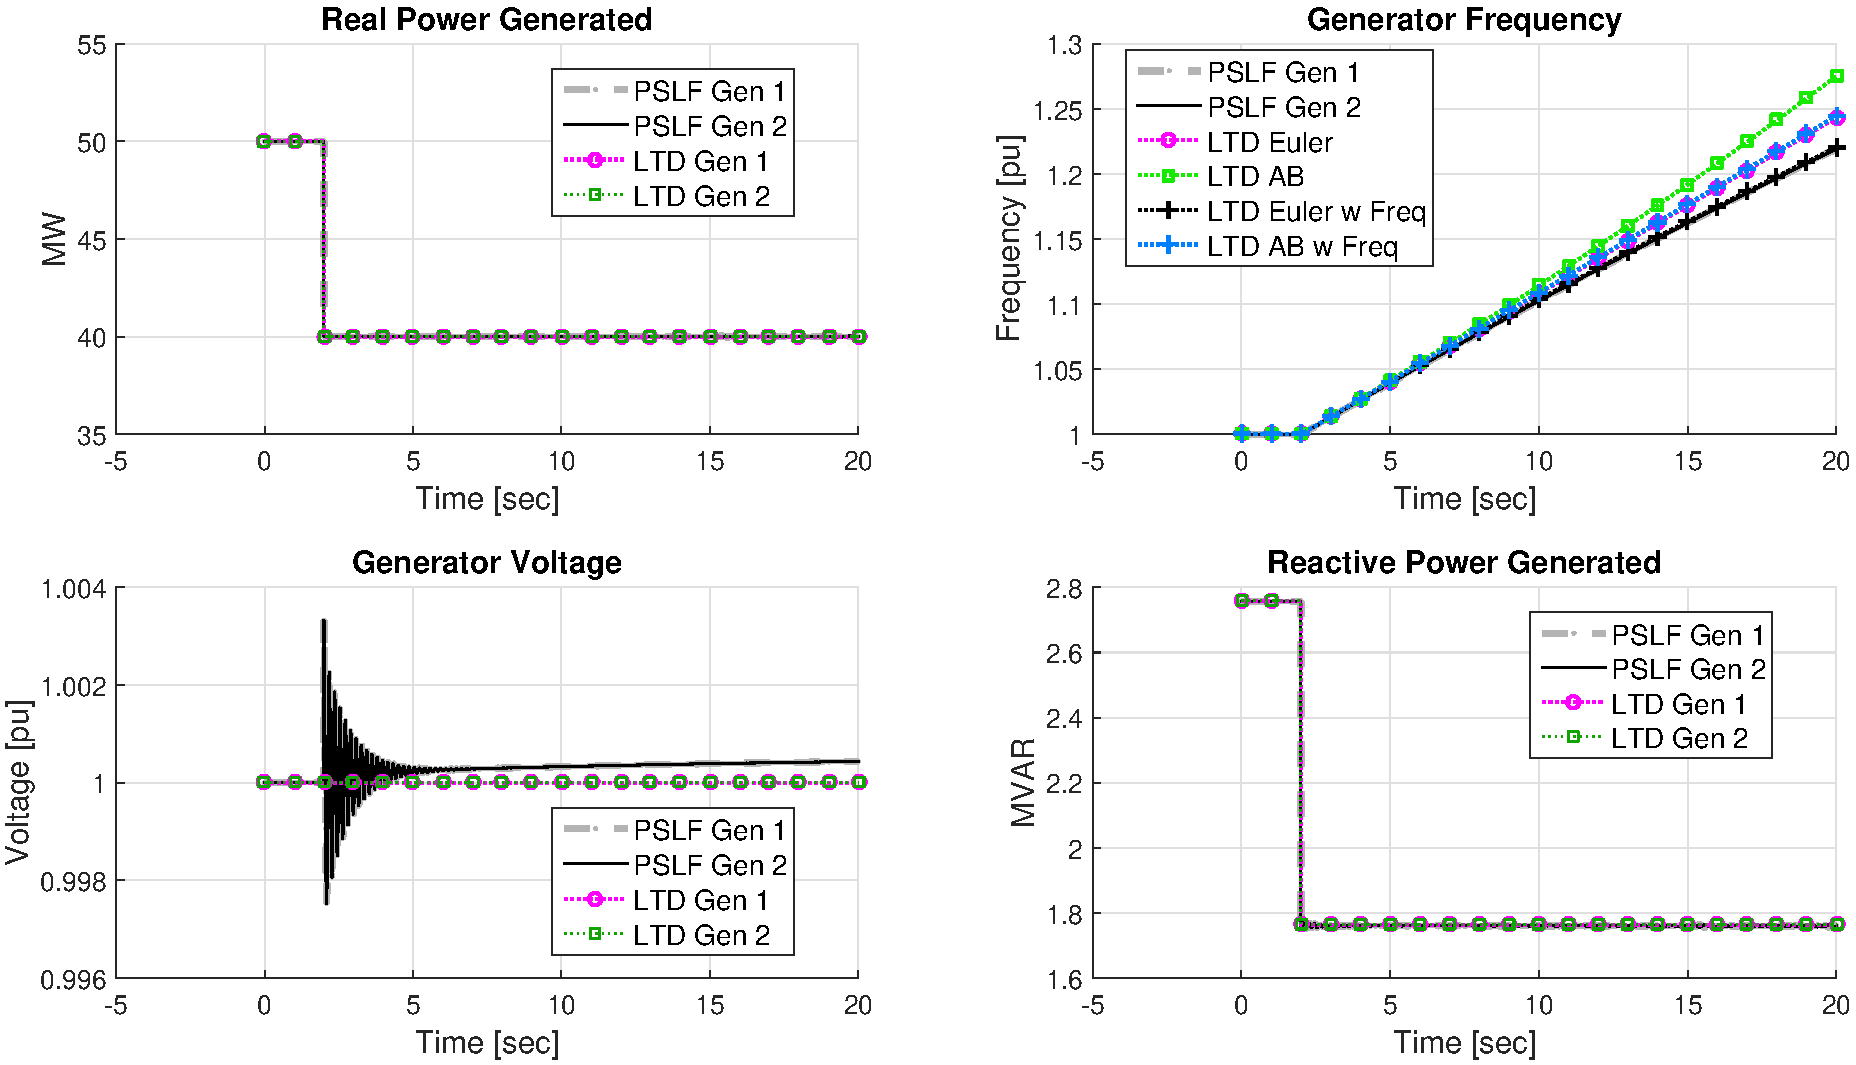
\includegraphics[width=\linewidth]{noGovExcLoadStepDsys}
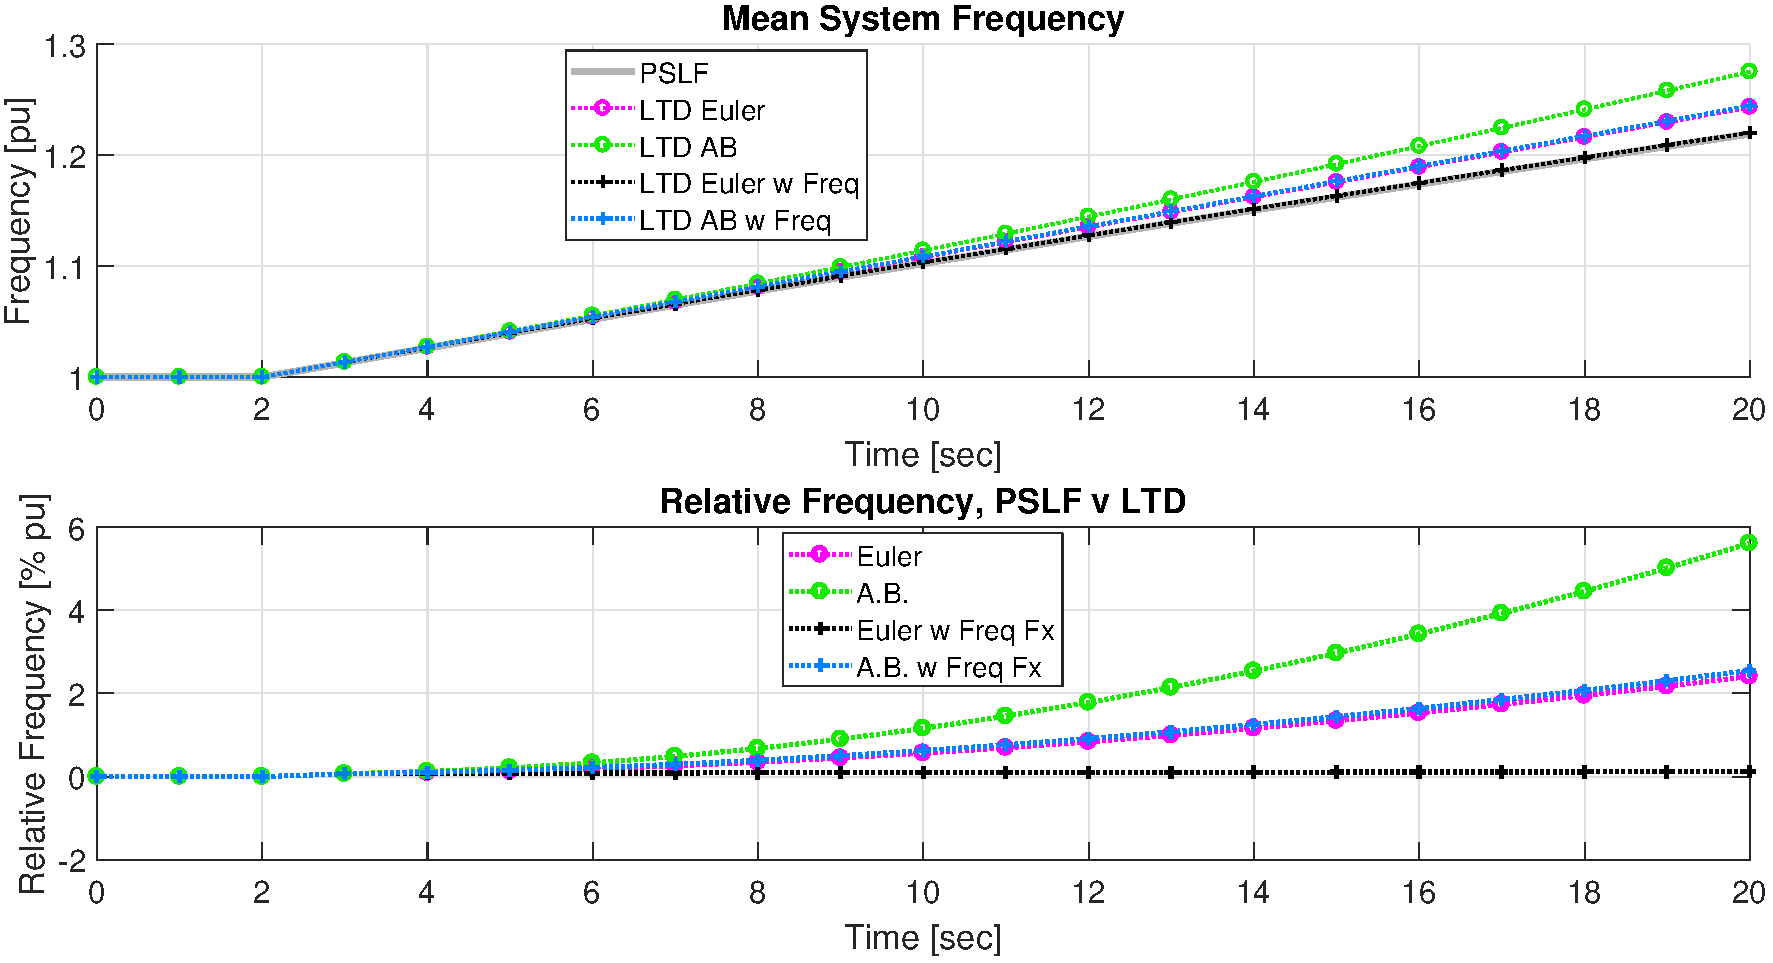
\includegraphics[width=\linewidth]{noGovExcLoadStepDfreq}
\pagebreak

\paragraph{pgov1 Tests:}Stepping 20 MW of load down at t=2, then 30 MW up at t=32.\\
pgov1 on only gen 1:  \vspace{1em}\\
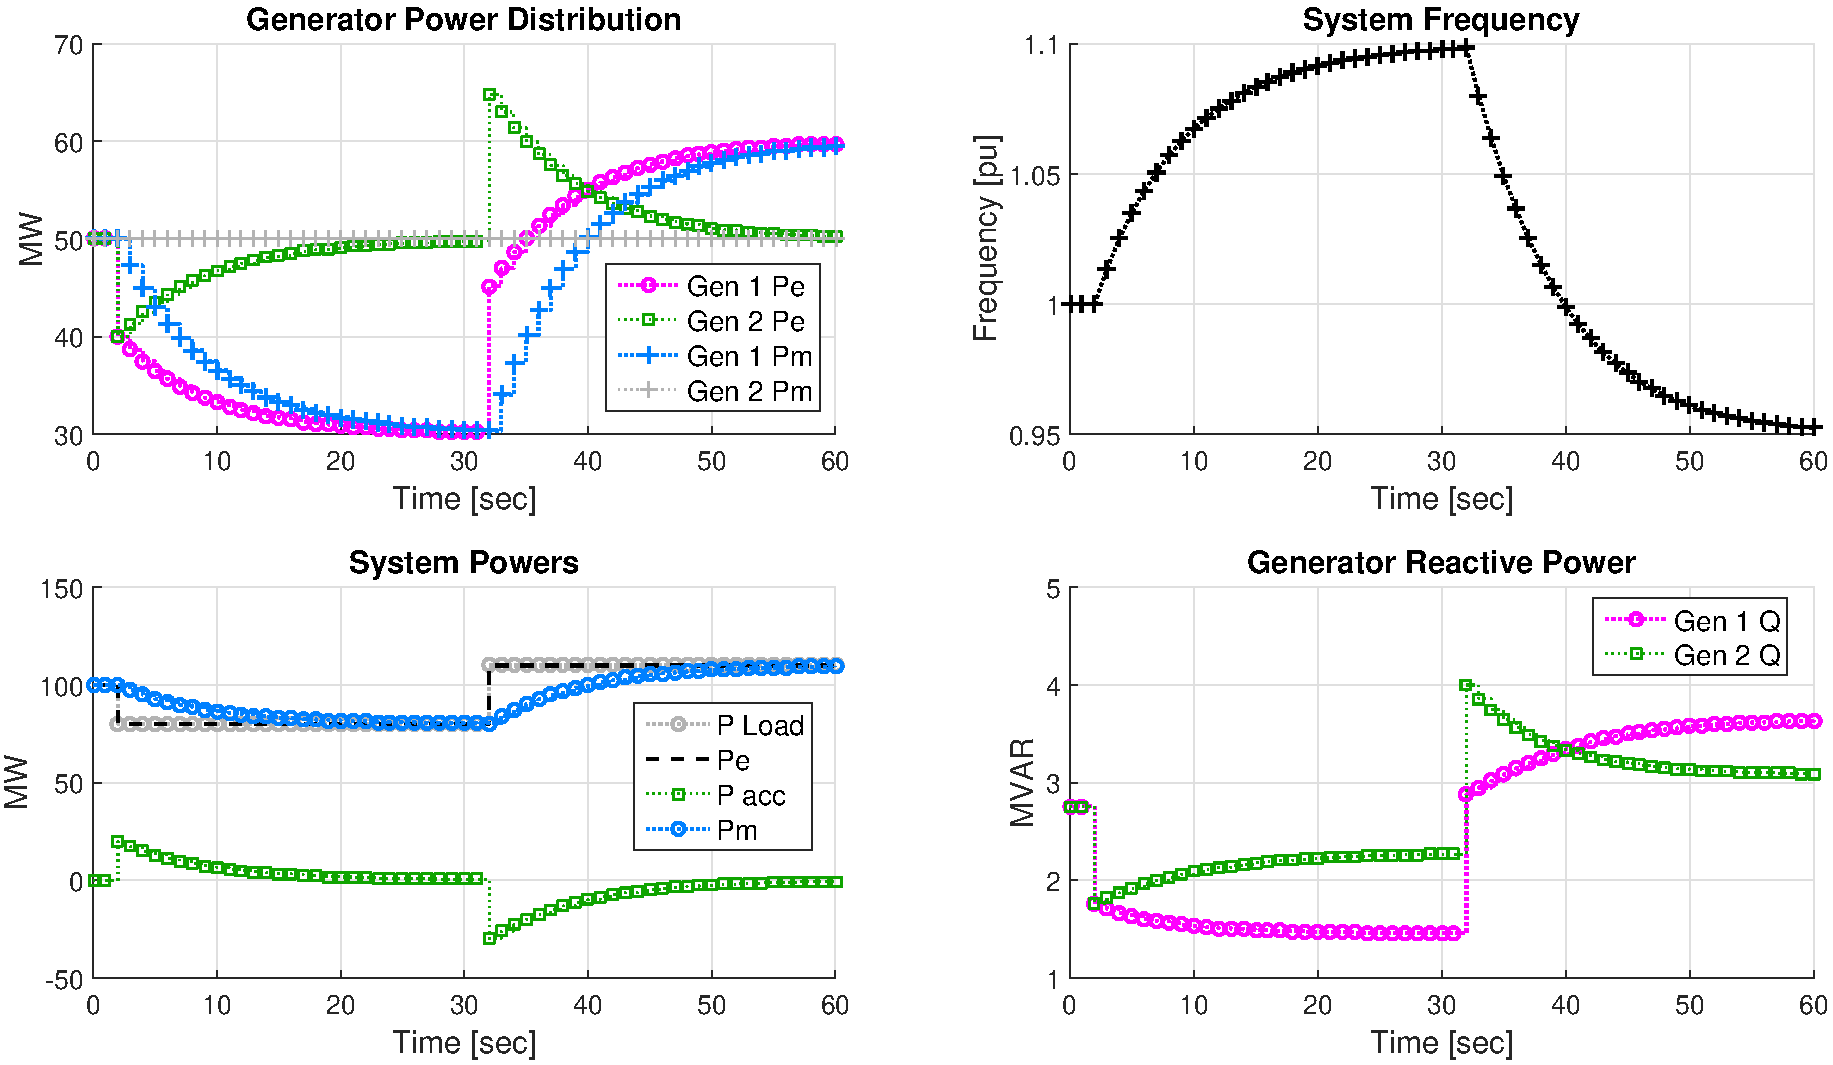
\includegraphics[width=\linewidth]{pgov1x1}
pgov1 on both gens:\\
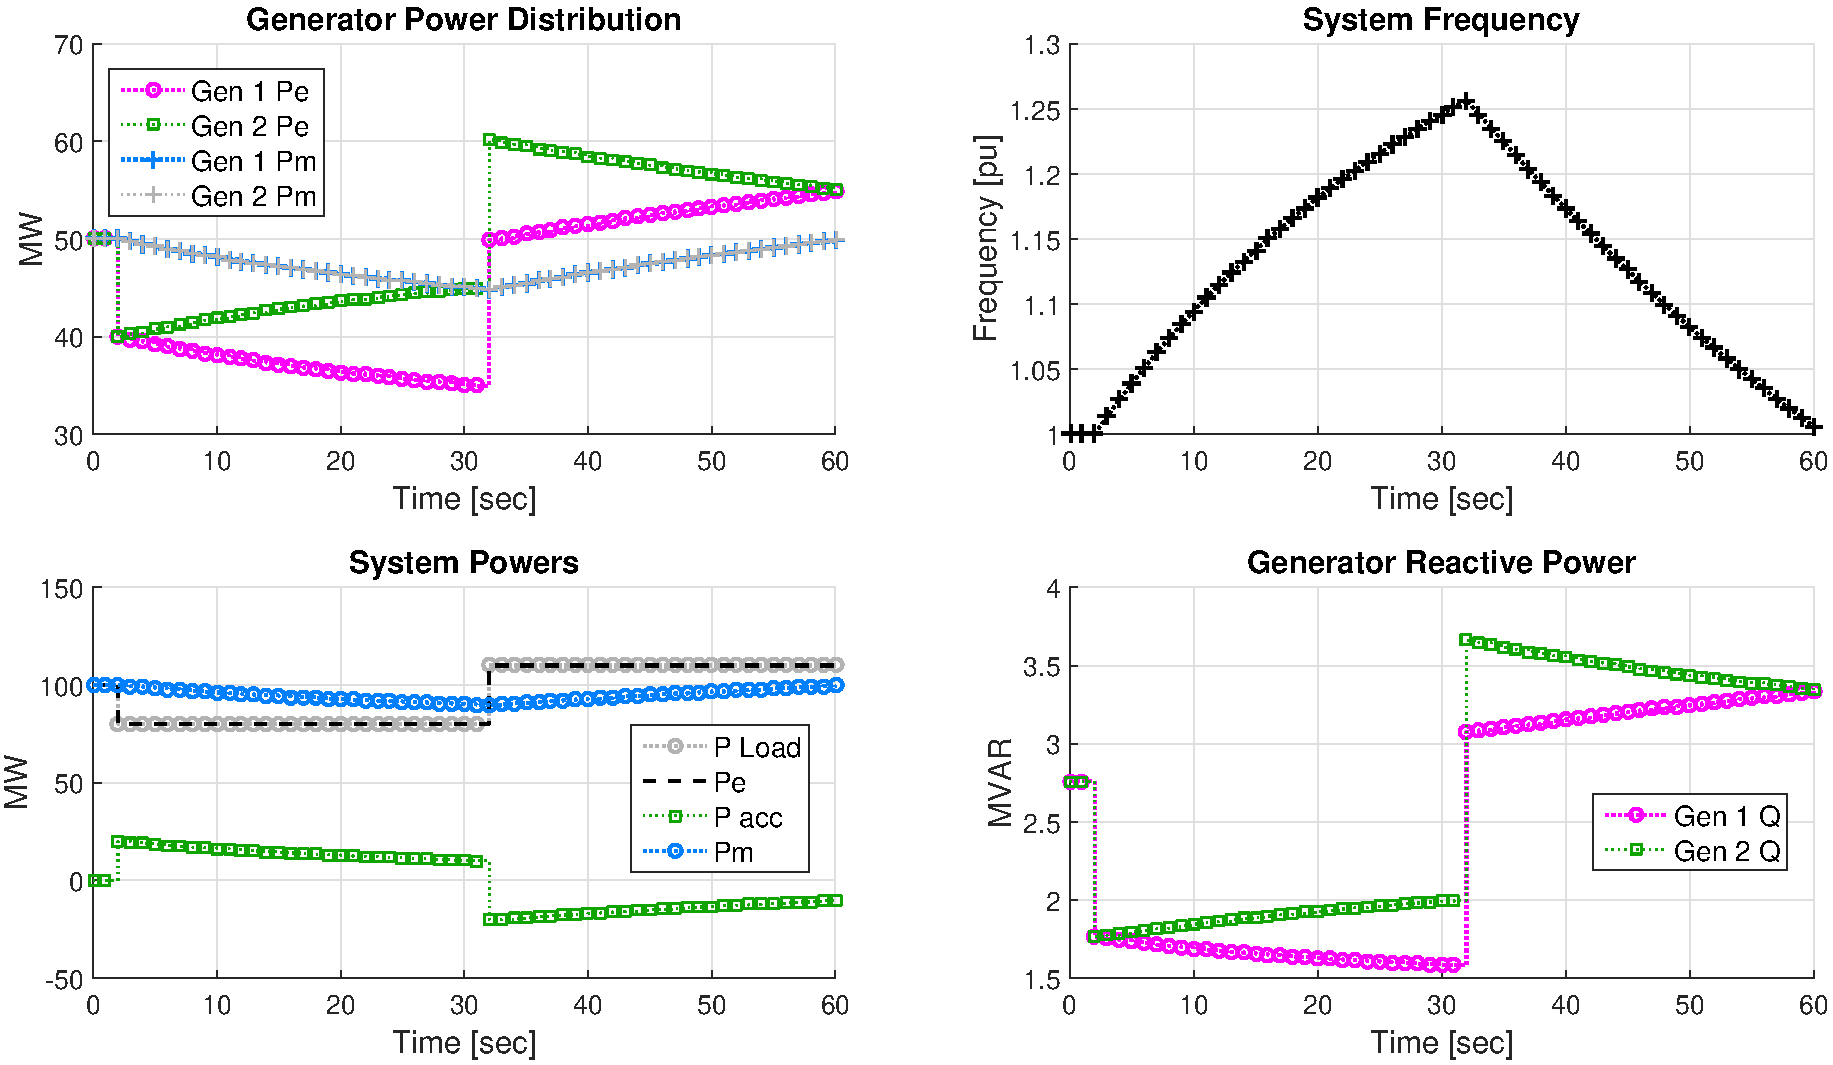
\includegraphics[width=\linewidth]{pgov1x2}
	\end{comment}
\end{document}